\documentclass[conference]{IEEEtran}

\usepackage{graphicx}
\usepackage[T1]{fontenc}
\usepackage[utf8]{inputenc}
\usepackage{lmodern}
\usepackage{amsmath}
\usepackage{booktabs}
\usepackage{hyperref}
\usepackage{listings}
\usepackage{tikz}
\usepackage{float}
\usetikzlibrary{positioning,shapes.geometric,fit}

\hypersetup{
    colorlinks=true,
    linkcolor=black,
    urlcolor=blue,
    citecolor=black
}

\lstset{
    basicstyle=\ttfamily\scriptsize,
    breaklines=true,
    frame=single,
    columns=fullflexible,
    keepspaces=true,
    showstringspaces=false
}

\title{Tarif Rehberi Uygulaması\\
\large Kocaeli Üniversitesi Bilgisayar Mühendisliği Bölümü\\
Yazılım Laboratuvarı I}

\author{
\IEEEauthorblockN{Alper Aydın -- 190201064\\190201064@kocaeli.edu.tr}
\IEEEauthorblockA{Kocaeli Üniversitesi, Bilgisayar Mühendisliği Bölümü\\
Yazılım Laboratuvarı I}
}

\begin{document}
\maketitle

\begin{abstract}
Bu çalışmada, kullanıcıların yemek tariflerini saklayabildiği, tariflerde kullanılan malzemeleri yönetebildiği ve elde bulunan malzemelere göre uygun tarifleri inceleyebildiği bir masaüstü uygulaması geliştirilmiştir. Süre kısıtı nedeniyle geliştiricinin iyi bildiği ve rahat çalıştığı Python tercih edilmiş, grafik arayüz PySide6 ve veritabanı SQLite ile oluşturulmuştur. Uygulama tarif ve malzeme ekleme, güncelleme ve silme; tarif-malzeme ilişkilerini yönetme; dinamik arama, filtreleme ve sıralama; tarif maliyeti ve eksik malzeme maliyeti hesaplama; malzeme yeterliliği; eşleşme yüzdesine göre tarif önerme işlevlerini içermektedir. Yazılım model, repository, service ve GUI katmanlarına ayrılmıştır.
\end{abstract}

\begin{IEEEkeywords}
Tarif Rehberi, Python, PySide6, SQLite, masaüstü uygulama, dinamik filtreleme, tarif önerme, UML
\end{IEEEkeywords}

\section{Giriş}
Projenin amacı, kullanıcının yemek tariflerini veritabanında saklayabildiği ve elindeki mevcut malzemelere göre hangi tariflerin hazırlanabileceğini görebildiği bir masaüstü uygulaması geliştirmektir. Gereksinimler; veritabanı yönetimi, dinamik arama ve filtreleme, sıralama, maliyet hesaplama, algoritmik değerlendirme ve kullanıcı dostu grafik arayüzün birlikte gerçekleştirilmesini gerektirmektedir.

Geliştirme sürecindeki temel yaklaşım, verilen süre içinde doğrudan proje gereksinimlerine karşılık veren çalışan ve test edilebilir bir uygulama ortaya koymaktır. Bu nedenle teknoloji seçimi yapılırken yalnızca teorik olarak mümkün seçenekler değil, geliştirme hızı, mevcut bilgi birikimi ve proje için gerçek teknik ihtiyaçlar dikkate alınmıştır.

\section{Yöntem}

\subsection{Teknoloji Seçimi}
Proje için Python tercih edilmesinin temel nedeni süre kısıtıdır. Süre içerisinde hızlı ve kontrollü sonuç verebilmek amacıyla iyi bilinen ve rahat çalışılınan bir programlama dili olduğu için seçilmiştir. Yeni bir programlama dili ve geliştirme ekosistemi öğrenmek yerine mevcut Python bilgisinden yararlanılması, zamanın doğrudan uygulama işlevlerine ayrılmasını sağlamıştır.

Ödev kapsamında Java veya C\# kullanılması istenmiş olsa da, bu proje özelinde Java için JVM ve C\# için .NET/CLR kullanımının gerekli bir avantaj sağlamadığı değerlendirilmiştir. Projede gereken veritabanı işlemleri, tarif-malzeme ilişkileri, filtreleme, maliyet hesabı, öneri algoritması ve masaüstü arayüzü Python ile doğrudan gerçekleştirilebilmiştir. Dolayısıyla burada alınan karar, Java veya C\#'ın yetersiz olduğu yönünde değil; süre sınırı içinde yeni bir ekosisteme geçmenin bu proje için ölçülebilir bir fayda oluşturmadığı yönündedir.

Grafik kullanıcı arayüzü için PySide6 seçilmiş, veritabanı olarak ayrı bir sunucu gerektirmeyen SQLite kullanılmıştır. Uygulama başlangıcında veritabanı şeması oluşturulmakta ve ardından PySide6 uygulaması başlatılmaktadır.

\subsection{Yazılım Mimarisi}
Kod, model, repository, service ve GUI sorumluluklarını ayırmaktadır. \textit{Recipe} ve \textit{Ingredient} sınıfları temel veri yapılarını temsil etmektedir. Repository katmanı SQLite sorgularını yürütmektedir. Service katmanında tarif eşleşmesi, eksik malzemeler, maliyet ve öneri algoritmaları bulunmaktadır. GUI katmanında ise \textit{MainWindow} ile tarif ve malzeme yönetimi ekranları bulunmaktadır.

Tarif-malzeme ilişkisi kodda ayrı bir Python model sınıfı olarak değil, SQLite içindeki \texttt{recipe\_ingredients} tablosu üzerinden tutulmaktadır. Bu tabloda tarif kimliği, malzeme kimliği ve tarifte gereken miktar bulunmaktadır. Veritabanı şemasında ayrıca tarif ve malzeme adlarının benzersiz olması, miktarların geçerli aralıkta bulunması ve yabancı anahtar ilişkilerinin korunması için kısıtlamalar bulunmaktadır.

\begin{figure*}[t]
	\centering
	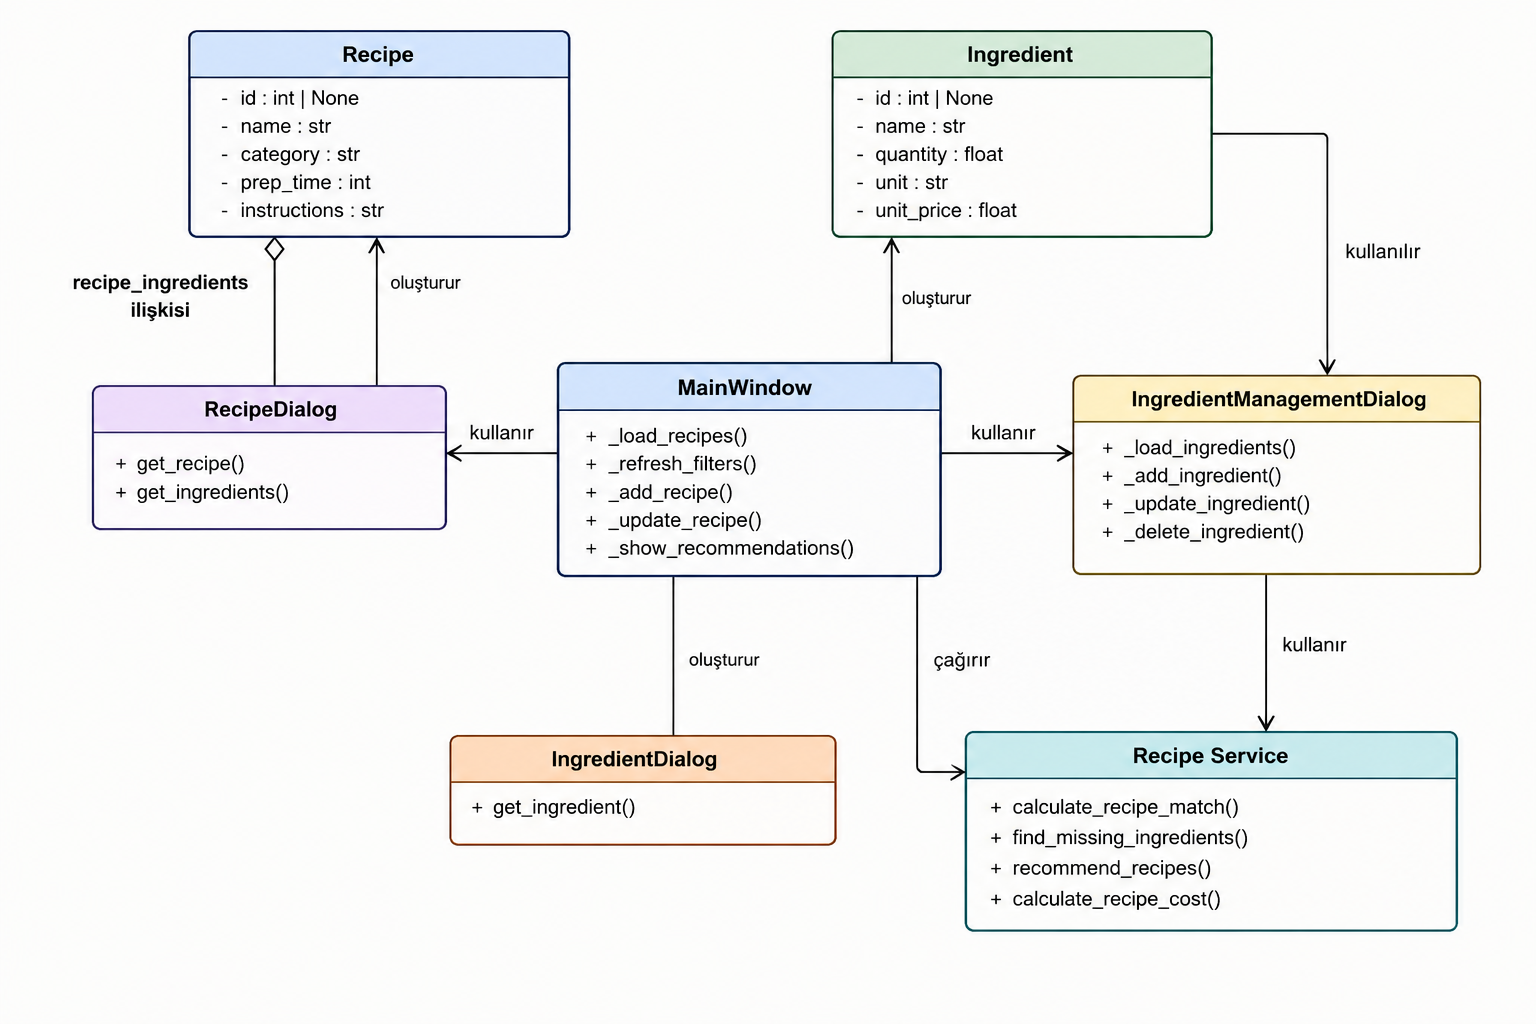
\includegraphics[
	width=0.92\textwidth
	]{UML.png}
	\caption{Gerçekleştirilen uygulamanın UML sınıf diyagramı}
	\label{fig:uml}
\end{figure*}

\subsection{Kullanıcı Arayüzü}
Ana pencere tarif adı araması, kategori seçimi, malzeme araması, malzeme sayısı sınırları, maliyet sınırları ve sıralama seçeneklerini içermektedir. Tarif listesinde seçili tarifin ayrıntıları gösterilmekte; tarifin maliyeti, malzemeleri, eksik malzeme maliyeti ve yapılışı görüntülenmektedir. Tarif ekleme ve güncelleme ekranında malzemeler ``Malzeme=Miktar'' biçiminde girilebilmektedir. Örneğin ``Domates=3'' ifadesi, tarifin üç birim domatese ihtiyaç duyduğunu belirtmektedir.

Ayrı malzeme yönetimi ekranında malzeme adı, stok miktarı, birim ve birim fiyatı yönetilmektedir. Tarif oluşturulurken girilen malzeme mevcut değilse servis katmanındaki \texttt{create\_ingredient\_if\_not\_exists} işlevi ile oluşturulmakta, mevcutsa mevcut kayıt kullanılmaktadır.

\section{Algoritma}

Uygulamanın temel algoritması, kullanıcının mevcut malzemeleri ile tarifte gerekli olan malzemeleri karşılaştırarak tarifin eşleşme yüzdesini hesaplamak ve sıfırdan büyük eşleşme sağlayan tarifleri yüzdelerine göre sıralamaktır. Gerçek servis kodunda \texttt{calculate\_recipe\_match} önce ilgili tarifin malzemelerini almaktadır. Tarif malzemelerinin tamamı dolaşılarak kullanıcının sahip olduğu miktarın gerekli miktardan büyük veya eşit olup olmadığı kontrol edilmektedir. Yeterli olan malzeme sayısı toplam malzeme sayısına bölünmekte ve 100 ile çarpılmaktadır.

Eşleşme yüzdesi:
\begin{equation}
M = \frac{Y}{T}\times100
\end{equation}
Burada $T$ tarifteki toplam malzeme sayısını, $Y$ ise miktarı yeterli olan malzemelerin sayısını göstermektedir. Tarifin malzeme listesi boşsa sonuç $0$ olarak döndürülmektedir.

\texttt{recommend\_recipes} fonksiyonu bütün tarifleri alır, her tarif için yukarıdaki eşleşme yüzdesini hesaplar, yüzdesi sıfır olmayanları sonuç listesine ekler ve önce yüzde azalan, eşit durumda tarif adı artan şekilde sıralar. Ayrıca \texttt{find\_missing\_ingredients} gerekli miktarı karşılamayan malzemeleri ayrı olarak belirlemektedir. Tarif maliyeti ise her malzemenin birim fiyatı ile tarifte gerekli miktarının çarpımlarının toplamı olarak hesaplanmaktadır.

Bu algoritmada $n$ tarif ve her tarifte ortalama $m$ malzeme olduğu varsayılırsa eşleşme hesaplamasının zaman karmaşıklığı yaklaşık $O(nm)$'dir. Projenin masaüstü kullanım senaryosunda kullanılan veri miktarı için bu yaklaşım yeterlidir ve anlaşılır bir uygulama mantığı sağlamaktadır.

\begin{figure*}[t]
	\centering
	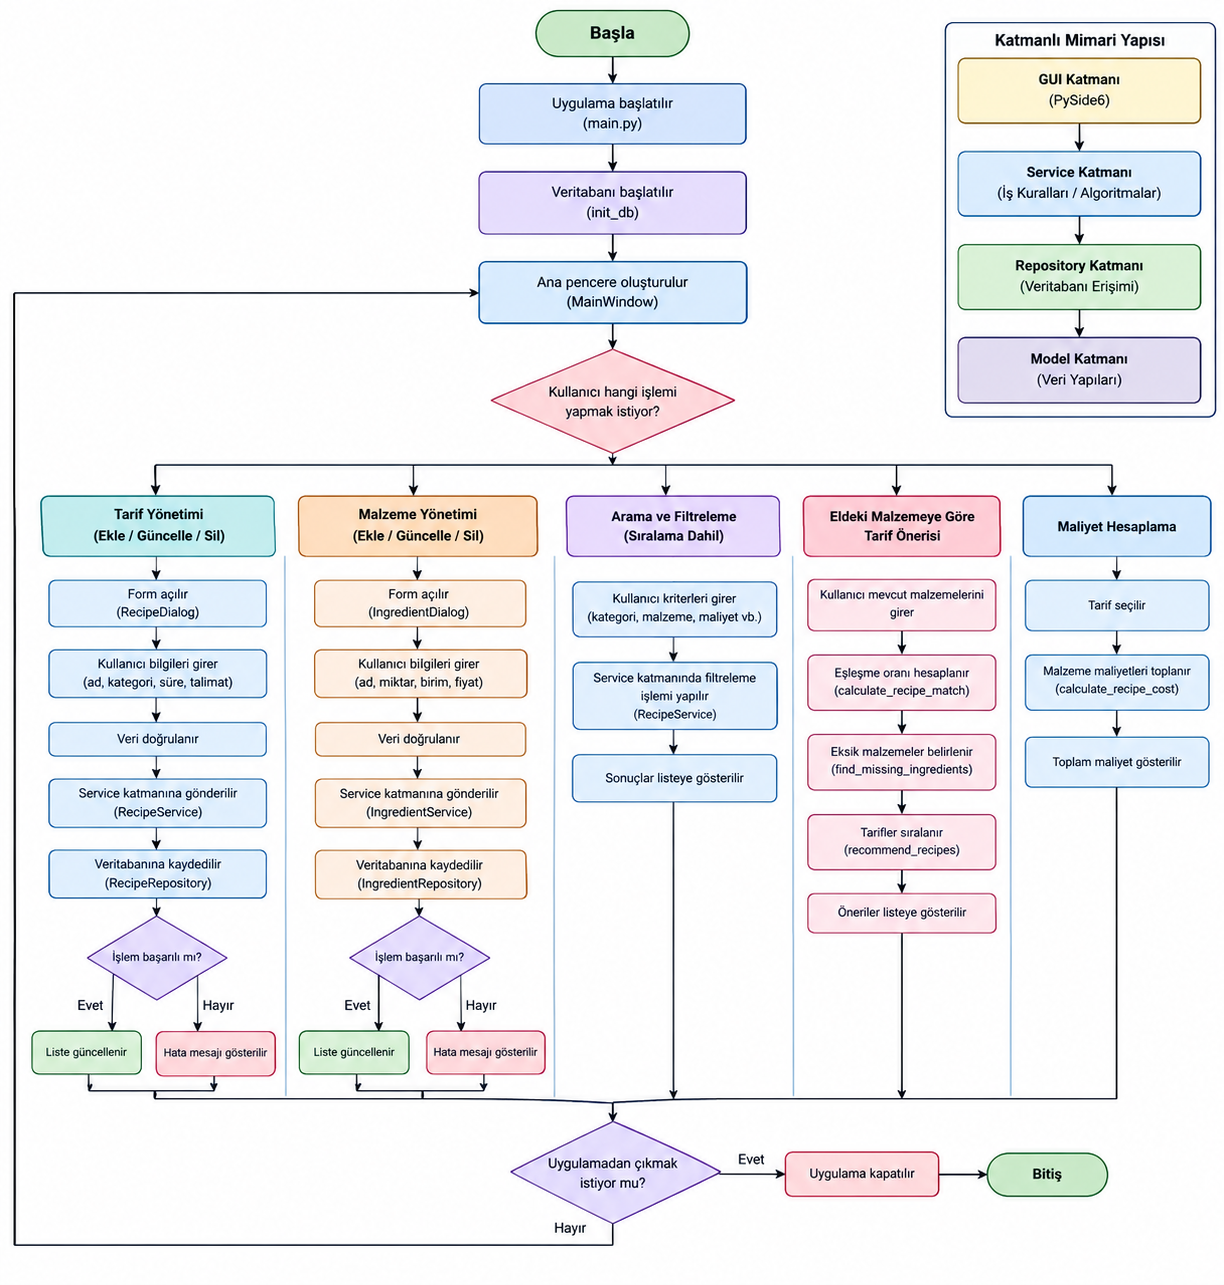
\includegraphics[
	width=0.92\textwidth
	]{Akış.png}
	\caption{Tarif Rehberi uygulamasının genel akış diyagramı}
	\label{fig:flowchart}
\end{figure*}
\section{Deneysel Sonuçlar}
Geliştirme sırasında repository ve service katmanları için veri ekleme, güncelleme, silme, maliyet hesaplama, malzeme eşleşmesi ve tarif önerme davranışları test edilmiştir. GUI geliştirilirken ana pencerenin oluşturulması, gerekli giriş alanlarının ve düğmelerin bulunması, tariflerin yüklenmesi, tarif ayrıntılarının gösterilmesi ve yeterlilik durumunun arayüzde yansıtılması doğrulanmıştır.

Test ortamında gerçek veritabanından ayrı geçici SQLite dosyalarının kullanılması ile testlerin birbirini etkilememesi sağlanmıştır. Bu yöntem özellikle veritabanı katmanındaki CRUD işlemlerinin güvenli biçimde doğrulanmasına yardımcı olmuştur.

Uygulamada toplam 10 örnek tarif kullanılmış ve bu tarifler beşten fazla kategoriye dağıtılmıştır. Ana Yemek, Çorba, Atıştırmalık, Salata, Pilav, Kahvaltı ve Tatlı kategorileri örnek veri kümesinde bulunmaktadır. Test amacıyla Menemen, Mercimek Çorbası, Kıymalı Makarna, Patates Kızartması, Tavuk Sote, Çoban Salata, Pilav, Omlet, Sütlaç ve Krep tarifleri kullanılmıştır.

Arayüzde mevcut tüm malzemeleri yeterli olan tarifler yeşil, en az bir malzemesi eksik olan tarifler kırmızı gösterilmektedir. Tarif detayında toplam maliyet ve eksik miktarların maliyeti hesaplanmaktadır. Malzeme adına göre filtreleme yapıldığında eşleşen tarifler arasındaki oran da kullanıcıya gösterilmektedir.

\clearpage
\section{Sonuç}
Bu çalışmada tarif ve malzemelerin yönetilebildiği, tarif-malzeme ilişkilerinin veritabanında tutulduğu ve mevcut malzemelere göre tariflerin değerlendirilebildiği bir masaüstü uygulaması gerçekleştirilmiştir. Uygulamanın kapsamı doğrudan proje gereksinimlerine odaklanacak şekilde tutulmuş, gereksiz ek özelliklerle genişletilmemiştir.

Python ve PySide6 seçimi, süre kısıtı altında iyi bilinen bir teknoloji ile hızlı ve kontrollü ilerleme amacıyla yapılmıştır. Java için JVM ve C\# için .NET/CLR gibi çalışma ortamlarının proje özelinde zorunlu veya belirgin bir teknik avantaj sağlamadığı değerlendirilmiş ve mevcut Python bilgisi kullanılarak zamanın doğrudan uygulama işlevlerine ayrılması tercih edilmiştir.

Gerçekleştirilen eşleşme algoritması, tariflerin mevcut malzemelere ne ölçüde uyduğunu sayısal olarak ifade etmekte ve öneri mekanizmasının temelini oluşturmaktadır. UML diyagramı uygulamadaki temel sınıfların ve kullanım ilişkilerinin yapısını, akış diyagramı ise öneri algoritmasının çalışma sürecini göstermektedir. Böylece yazılımın yalnızca çalışan kodu değil, tasarım ve algoritma mantığı da dokümante edilmiştir.

\begin{thebibliography}{00}
\bibitem{python} Python Software Foundation, ``Python Documentation,'' \url{https://docs.python.org/3/}.
\bibitem{pyside} Qt for Python, ``PySide6 Documentation,'' \url{https://doc.qt.io/qtforpython-6/}.
\bibitem{sqlite} SQLite, ``SQLite Documentation,'' \url{https://www.sqlite.org/docs.html}.
\bibitem{pytest} pytest Development Team, ``pytest Documentation,'' \url{https://docs.pytest.org/}.
\bibitem{ieee} IEEE, ``IEEE Author Center,'' \url{https://ieeeauthorcenter.ieee.org/}.
\end{thebibliography}

\end{document}
